\documentclass[10pt,a4paper,onecolumn]{article}
\usepackage[usenames,dvipsnames]{color}
\usepackage[colorlinks,citecolor=blue]{hyperref}
\usepackage{appendix}
% we need umlauts in the refs
\usepackage[english]{babel}
\usepackage[utf8]{inputenc}
\usepackage[T1]{fontenc}

%\usepackage[natbib=true,style=authoryear,backend=biber]{biblatex}
\usepackage{authblk}
\renewcommand\Affilfont{\itshape\small}
\usepackage{graphicx}
\usepackage[authoryear]{natbib}
\usepackage{url}
\usepackage{todonotes}
%\usepackage{endfloat}
% nicer units
\usepackage{units}
% better tables
\usepackage{booktabs}
% Some colorings for the tables
%\usepackage[table]{xcolor}

%\usepackage{multirow}

% switch for final stage
%\graphicspath{{pics/}}
\graphicspath{{pics/}
              {pics/generated/}}

%\usepackage{lineno}
%\usepackage[leftbars]{changebar}
%\setlength\changebarsep{0.5em}
%\usepackage{comment}

%\usepackage[space]{grffile}
%\usepackage{latexsym}
%\usepackage{amssymb}
%\usepackage{fancyref}
\usepackage{textcomp}

\usepackage{marvosym}
\usepackage{listings}

\lstset{prebreak=\Righttorque}
\lstset{postbreak=\Lefttorque}
\lstset{breakindent=0pt}
\lstset{frame=lines}
\lstset{aboveskip=4mm}
\lstset{breaklines=true, breakatwhitespace=false}
\urlstyle{same}
% howto cite projects
\newcommand{\purl}[2]{#1\footnote{\url{#2}}}

\newcommand{\sevenT}{\unit[7]{Tesla}}
\newcommand{\threeT}{\unit[3]{Tesla}}
\newcommand{\mm}[1]{\unit[#1]{mm}}
\newcommand{\seconds}[1]{\unit[#1]{s}}

\newcommand{\ie}[0]{\emph{i.e.},\ }
\newcommand{\eg}[0]{\emph{e.g.},\ }
\newcommand{\etc}[0]{\emph{etc.}}

\begin{document}
\bibliographystyle{unsrtnat}

\title{Decoding musical genre with an fMRI encoding model of musical
features -- a 3T/7T comparison}


\author[1]{Moritz~Boos}
\author[2]{J.~Swaroop~Guntupalli}
\author[3,4]{Michael~Hanke}

\affil[1]{Oldenburg, Germany}
\affil[2]{Department of Psychological and Brain Sciences,
  Dartmouth College, Hanover, New Hampshire, USA}
\affil[3]{Psychoinformatics lab, Department of Psychology II, University of
Magdeburg, Magdeburg, Germany}
\affil[4]{Center for Behavioral Brain Sciences, Magdeburg, Germany}
\maketitle
\thispagestyle{fancy}

\listoftodos

\begin{abstract}
% Abstracts should be up to 300 words and provide a succinct summary of the
% article. Although the abstract should explain why the article might be
% interesting, care should be taken not to inappropriately over-emphasise the
% importance of the work described in the article. Citations should not be used
% in the abstract, and the use of abbreviations should be minimized.

\todo[inline]{write abstract}
\end{abstract}

\clearpage


\section*{Introduction}


\todo[inline]{any fieldstrength differences, i.e. higher resolution gives better model?}
\todo[inline]{formisano says 7T better, but more stimuli and more data with a different model are confounds}
\todo[inline]{maybe add other feature sets and check metrics across all of them}

% summary: first comparative study

In functional magnetic resonance imaging (f{MRI}) research, voxel-wise encoding
models are an increasingly popular computational tool to characterize the
relationship between a real world stimulus and BOLD-activity patterns
\citep{NG11}\todo{if popular we need 2+ citations}.
%eigtl unnoetig
%Both stimulus and brain activity can be represented as high-dimensional vectors
%\cite{HCG14}, an encoding model is then trained separately for each voxel in a
%region of interest. 

Encoding models can be validated in a number of different ways: \citet{ML08},
for example, used a binary retrieval task to validate the predicted f{MRI}
images for the meaning of nouns, while \citet{KG+08} used stimulus
identification, and \citet{NG09} used \todo{quality of?}stimulus reconstruction
as quality metrics.  In auditory neuroscience, where encoding models are less
frequent, only binary retrieval accuracy \citep{CTK+2012} and stimulus
identification \citep{SF14} have been used and it is yet unclear how the
results of these validation strategies vary with the parameters of f{MRI} data
analysis (e.g. number of voxels used)  or acquisition (e.g. field strength).
\citet{SF14} used stimulus identification to validate an encoding model for
natural sounds and reported a difference for 3-Tesla and 7-Tesla f{MRI} data,
although the different number of stimuli used in the two experiments might be a
potential confound.  Apart from field strength, researchers have also many
other degrees of freedom in constructing an encoding model.  Their choice of
parameters, like the number of voxels used, will affect the quality of
predictions, but it is unknown if these choices will affect encoding quality
metrics differentally.  Recently a 3-Tesla f{MRI} study on the perception of
musical genres \citep{CTK+2012} has been replicated with 7-Tesla data
\citep{HDH+2015}, making it possible to directly compare the effect of field
strength on different validation strategies for encoding models.  This study
aims to compare three quality metrics, binary retrieval accuracy \citep{ML08},
sound identification \citep{KG+08,SF14} and the decoding accuracy of a stimulus
feature, the musical genre. We do this by varying field strength, comparing
performance in a 3-Tesla and a 7-Tesla dataset, and two parameters of the data
analysis, the number of voxels used and how they were selected.  While we do
not replicate stimulus reconstruction as in \citep{NG09}, we use a similar
method of constructing a probabilistic decoding model from a set of
voxel-specific encoding models, and use it to infer the music genre of the
presented stimulus.
%possibly cite NG11


\section*{Methods}

\subsection*{fMRI data}

\paragraph{\unit[3]{Tesla}}
\paragraph{\unit[7]{Tesla}}

\citet{HDH+2015}; maybe \citet{HBI+14}

\subsection*{Encoding model}

\todo[inline]{feature representations citation}
%MPS??

To build an encoding model with high predictive power, we need to find an
appropriate feature representation of the music stimuli.  \citet{CTK+2012}
already compared different feature representations of the same stimuli in the
3T dataset. We chose the feature set with the best encoding performance in this
study, the low-quefrency mel-frequency spectrum (LQ-MFS) \citep{HDH+2015},
corresponding to the timbre of the stimulus. 


\missingfigure{encoding scheme}


For each f{MRI} sample $y_{vt}$ (where $t=1,2,..,T$ denotes the time-points and
$v=1,2,..,V$ denotes the voxels) the LQ-MFS features $x_{t}$ $[1x\widetilde{M}]$
(where $\widetilde{M}$ is the number of LQ-MFS coefficients) of the
corresponding two second part of the stimulus were computed. In case there was
no stimulus presented at time-point $t$, a zero vector $[1x\widetilde{M}]$ was
used. 

Since the BOLD response is delayed,  the most recent feature was vector removed
for each f{MRI} sample (since it could not yet have influenced the f{MRI}
activity), and the new feature vector at time-point $t$ was created by
concatenating the prior feature vectors $x_{t-1}$,$x_{t-2}$ and $x_{t-3}$. We
overload the notation and denote this stacked feature vector as $x_{t}$.
Feature vectors (and the corresponding f{MRI} sample) were removed from the
analysis, if two-thirds or more of the concatenated feature vectors were
zero-vectors.

The f{MRI} activity time-series, as well as the feature time-series, were
vertically stacked, resulting in a matrix of features $X$ $[NxM]$ (where $N$ is
the number of f{MRI} samples, and $M$ is number of LQ-MFS coefficients, with
$M=3\widetilde{M}$) and a matrix of f{MRI} activity $Y$ $[NxV]$ (where $V$ is
the number of voxels).

%probabilistic or objective function minimization, also cite someone about using lin. reg. in encoding
The encoding model could then be expressed as the probability to observe the f{MRI} activity at time-point $t$ and voxel $v$:
%
\begin{equation}
  \label{eq:encmo}
  p(y_{vt}|x_{t}) = N(y_{vt};x_{t}\beta_{v},\sigma)
\end{equation}
%
where $N(y;\mu,\sigma)$ denotes the probability density at point $y$ for a
gaussian with mean $\mu$ and standard deviation $\sigma$, and $\beta_{v}$ is a
$[Mx1]$ vector of regression coefficients specific to voxel $v$. To reduce
over-fitting the regression-coefficients were estimated using ridge regression
\citep{HK70}.  Independently for each voxel, the regularization parameter
$\lambda$ with the lowest mean squared error in a generalized leave-one-out
cross-validation \citep{GHW79} was chosen from a set of candidate values.

\subsection*{Quality metrics} \todo[inline]{add description of standardization}

\paragraph{Binary retrieval accuracy}

Binary retrieval accuracy \citep{ML08} estimates if a stimulus'
predicted f{MRI} activity is closer, in terms of cosine similarity, to its
observed f{MRI} activity than to the f{MRI} activity of a decoy stimulus.
This is done pair-wise for all combinations of stimuli and
then averaged.

%wiederholung.
In a prior study \citep{CTK+2012}, using the 3-Tesla data, binary retrieval
accuracy was used to validate voxel-specific encoding models on the same
dataset.

\paragraph{Correlation rank score}
%
An alternative measure of encoding performance is the correlation rank score or
matching score \citep{SF14}. For each stimulus $s_{n}$ in the validation set,
its predicted f{MRI} activity $\widetilde{y}_{n}$ is correlated with the
observed f{MRI} activity of every stimulus, $y_{i}$ for $i=1..25$. These
correlations are then ordered, and the  matching score $m(s_{n})$ is \[
m(s_{n}) = 1-\frac{rank(s_{n})-1}{N-1} \] Where $rank(s_{n})$ is the rank of
the correlation between predicted $\widetilde{y}_{n}$ and observed $y_{n}$
f{MRI} activity of $s_{n}$. Finally, the matching scores for all stimuli in the
validation set are averaged.

where $rank(s_{n})$ is the rank of the correlation between $\widetilde{i}_{n}$
and $i_{n}$.

Instead of testing the encoding performance, we can also test the performance of
a decoder based on the individual encoding models \citet{NG11}. To go from
$p(y_{vt}|x_{t})$ to $p(x_{t}|y_{t})$ we follow \citet{NG09} and first condense
the large number of voxel-specific encoding models into one multivoxel encoding model.
To do this we project the predicted and observed f{MRI} data onto the first $k$ principal components of the $[N x V]$ matrix of predicted f{MRI} activity \todo{Change to CV} (where $k$ is the number of principal components that retains 95\% of the variance and is chosen individually for each participant) 
%We do this by estimating the first $k$ principal components of the $[N x V]$ matrix of predicted f{MRI} activity \todo{Change to CV} (where $k$ is the number of principal components that retains 95\% of the variance and is chosen individually for each participant) and then projecting the predicted and measured f{MRI} activity onto them.
As in \citet{NG09} we construct the $k$-dimensional multivariate normal
probability density function $p(y_{t}|x_{t})$ and use a uniform prior
distribution $p(x_{t})$ to obtain the approximate posterior probability
$p(x_{t}|y_{t}) \propto p(y_{t}|x_{t})p(x_{t})$. Given the observed f{MRI}
activity we can now estimate the probability distribution over music stimuli
$p(s_{i}|y)$ (for $i=1..25$ (??)). We use the simplifying assumption that the
f{MRI} activity is influenced by the music stimuli only through their LQ-MFS
coefficients $x$, and - given that each music stimulus was associated with only
three (lagged) LQ-MFS representations - we arrive at $p(l_{i}|y) \propto
p(x_{t-1}|y_{t-1})p(x_{t}|y_{t})p(x_{t+1}|y_{t+1})$ where $t$ is the sample 6
seconds after the start of the music stimulus. The mode of this probability
distribution is the music stimulus that was most likely presented given the
observed f{MRI} activity. Since inter-genre similarity of LQ-MFS features drive
genre classification performance \citep{CTK+2012}, we predict the musical genre
of the presented stimulus given the observed f{MRI} activity as the mode of $p(c_{i}|y)
\propto \prod\nolimits_{l \in stim(c_{i})} p(l|y)$ where $stim(c_{i})$ are
the labels of the stimuli belonging to the genre $c_{i}$. 

\section*{Results}
%
\todo[inline]{number of voxels with other quality metrics} One of the degrees
of freedom was the number of voxels used in this analysis. \citet{ML08} chose
the 500 most stable voxels, while we evaluate the model performance for several
different number of voxels (see Figure \ref{fig:voxelnr}). In the further
analyses we use the best-performing number of voxel, i.e. 1000.

\begin{figure}
  \centering
  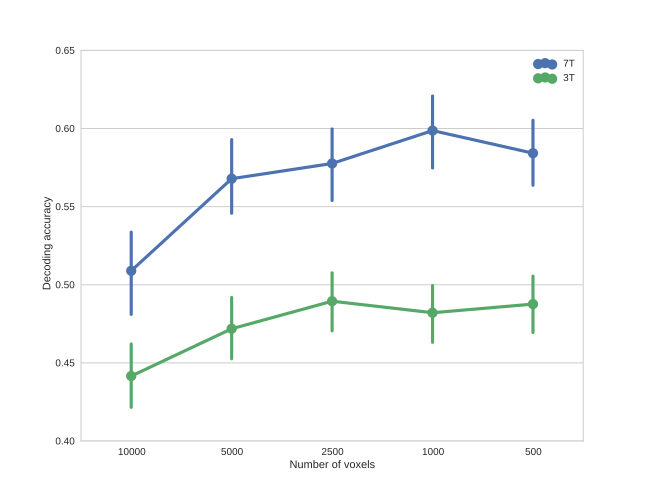
\includegraphics[width=\linewidth]{pics/nr_of_voxels_both}

  \caption{Mean decoding accuracy as a function of the included number of
  voxels for 3T and 7T. Error bars denote the bootstrapped 95\% confidence
  interval of the mean. The included voxels were the most stable ones i.e. their
  activity corresponding to each stimulus had the highest mean pairwise
  correlation across runs}

 \label{fig:voxelnr}
\end{figure}

%binary classification accuracy result, connect to casey/mitchel
\todo[inline]{potentially other nr of voxels, take avr across all runs for 3T and 7T}
\begin{figure}
  \centering
  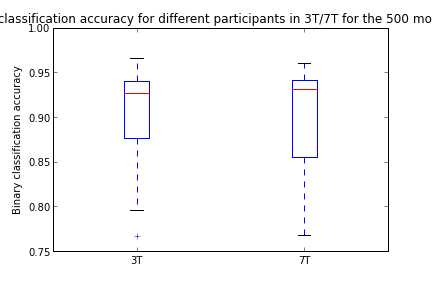
\includegraphics[width=\linewidth]{pics/binary_retrieval_accuracy}
  \caption{Binary retrieval classification accuracy for 3T and 7T}
  \label{fig:binretr}
\end{figure}

%correlation rankscore 3 and 7 incl. permutation analysis
\todo[inline]{potentially other nr of voxels, take avr across all runs for 3T and 7T,add permutation analysis}
\begin{figure}
  \centering
  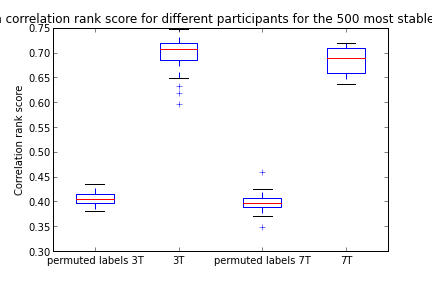
\includegraphics[width=\linewidth]{pics/correlation_rank_score}
  \caption{Correlation rank score for 3T and 7T}
  \label{fig:rankscore}
\end{figure}

%decoding(encoding) accuracy: 3 vs 7 (vs. plain decoding)
\todo[inline]{potentially other nr of voxels, take avr across all runs for 3T and 7T,add discriminative classifier baseline}
\begin{figure}
  \centering
  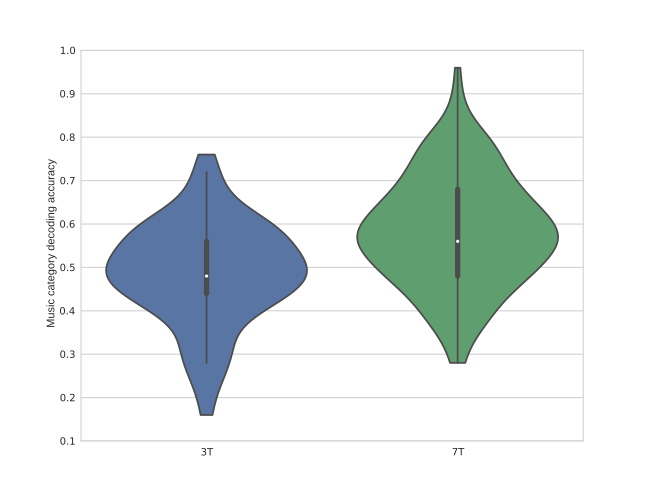
\includegraphics[width=\linewidth]{pics/decoding_accuracy}
  \caption{Decoding accuracy for 3T and 7T. A generative decoder was constructed by probabilistically inverting the encoding model.}
  \label{fig:decoder}
\end{figure}

\subsection*{Comparison of 3 and 7T}
%
\todo[inline]{Add words}
%
We compared the encoding performance between 3 and 7T for three different
quality metrics, binary retrieval accuracy (Figure \ref{fig:binretr}), a
correlation based matching score (Figure \ref{fig:rankscore}) and the decoding
accuracy for musical genres (Figure \ref{fig:decoder}). Each participant
contributed 8 datapoints to these violin plots (one for each held out run). The
first two metrics (which are purely encoding based) show a similar performance
for 3 and 7T, while decoding accuracy is higher for 7T. Decoding accuracy is
easily interpretable, it is harder to compare binary retrieval accuracy and the
matching score.     

\missingfigure{model validation on the movie}

\section*{Discussion}

We built an encoding model for LQ-MFS music features on a 3 and a 7T dataset,
and compared its performance using three different quality metrics, two of them
purely encoding based (binary retrieval accuracy and the correlation rank
matching score) and one using a decoding model built from our encoding model
(the decoding accuracy of each stimulus' music genre). We could show a similar
performance between 3 and 7T for the encoding based metrics, while the 7T led
to a higher decoding accuracy. Other studies \citep[e.g.,][]{SF14} found the opposite
effect using the matching score, but their 3T and 7T datasets did also differ
in the number of stimuli used. Interestingly, encoding in 7T became
advantageous if we used it to decode a stimulus feature (the music genre). To
do this we combined the single voxel encoding models into a multivoxel encoding
model \citep[see][]{NG09}, reducing the dimensionality of our model to gain a
more stable estimate. Should the voxels selected by a stability criterion in 7T
be actually more heterogeneous (e.g. mixing LQ-MFS sensitive voxels with
non-sensitive ones) than the ones selected in 3T, this could mitigate the
effect of the higher functional contrast-to-noise ratio in 7T, but might not
matter if we reduce the massive single voxel encoding to a multivoxel encoding
model.

%pretty speculative, add citations...
Of the three quality metrics used, binary retrieval accuracy and the
correlation rank score are maximized by an encoding model with high predictive
power (that explains much of the variance of the f{MRI} data) and a high
variance in the feature set of the predictors (even with strong predictive
power, the predictions need to differ for high scores in these metrics).
Additionally, for a high decoding accuracy (in a generative decoder) the
feature set needs to covary with the stimulus labels and the relationship
between stimulus and f{MRI} activity needs to be conditional on the chosen
feature set. In contrast to a discriminative decoder, this not only tests how
well a stimulus label is recoverable, but also how well the stimulus label is
encoded by this particular feature set.

%look Wehbe 2014 up again
All encoding models were trained to predict the (pre-processed) f{MRI}
time-series without explicitly modelling the BOLD response. 


\todo[inline]{decode(encode(fmri)) vs. plain decoding}

\todo[inline]{naturalistic validation is now mandatory}


\section*{Author contributions}
%In order to give appropriate credit to each author of an article, the
%individual contributions of each author to the manuscript should be detailed
%in this section. We recommend using author initials and then stating briefly
%how they contributed.

MB performed the analysis and wrote the manuscript.
JSG contributed to the manuscript.
MH contributed to the manuscript.


\section*{Competing Interests}
No competing interests were disclosed.

\section*{Grant Information}

This research was, in part, supported by the German Federal Ministry of
Education and Research (BMBF) as part of a US-German collaboration in
computational neuroscience (CRCNS; awarded to James Haxby, Peter Ramadge, and
Michael Hanke), co-funded by the BMBF and the US National Science Foundation
(BMBF 01GQ1112; NSF 1129855).  Work on the data-sharing technology employed for
this research was supported by US-German CRCNS project awarded to
Yaroslav~O.~Halchenko and Michael~Hanke, co-funded by the BMBF and the US
National Science Foundation (BMBF 01GQ1411; NSF 1429999).  Michael Hanke was
supported by funds from the German federal state of Saxony-Anhalt, Project:
Center for Behavioral Brain Sciences.


\section*{Acknowledgements}
%This section should acknowledge anyone who contributed to the research or the
%article but who does not qualify as an author based on the criteria provided
%earlier (e.g. someone or an organisation that provided writing assistance).
%Please state how they contributed; authors should obtain permission to
%acknowledge from all those mentioned in the Acknowledgements section.  Please
%do not list grant funding in this section (this should be included in the
%Grant information section - See above).

We are grateful to Michael Casey\ldots

\todo[inline]{express gratitude}

\bibliography{references}
\end{document}

% vim: textwidth=80 colorcolumn=81
